% Options for packages loaded elsewhere
\PassOptionsToPackage{unicode}{hyperref}
\PassOptionsToPackage{hyphens}{url}
\PassOptionsToPackage{dvipsnames,svgnames,x11names}{xcolor}
\PassOptionsToPackage{space}{xeCJK}
\documentclass[
  10pt,
]{article}
\usepackage{xcolor}
\usepackage[margin=0.65in]{geometry}
\usepackage{amsmath,amssymb}
\setcounter{secnumdepth}{-\maxdimen} % remove section numbering
\usepackage{iftex}
\ifPDFTeX
  \usepackage[T1]{fontenc}
  \usepackage[utf8]{inputenc}
  \usepackage{textcomp} % provide euro and other symbols
\else % if luatex or xetex
  \usepackage{unicode-math} % this also loads fontspec
  \defaultfontfeatures{Scale=MatchLowercase}
  \defaultfontfeatures[\rmfamily]{Ligatures=TeX,Scale=1}
\fi
\usepackage{lmodern}
\ifPDFTeX\else
  % xetex/luatex font selection
  \setmainfont[]{Arial}
  \setmonofont[]{Consolas}
  \ifXeTeX
    \usepackage{xeCJK}
    \setCJKmainfont[]{Microsoft YaHei}
  \fi
  \ifLuaTeX
    \usepackage[]{luatexja-fontspec}
    \setmainjfont[]{Microsoft YaHei}
  \fi
\fi
% Use upquote if available, for straight quotes in verbatim environments
\IfFileExists{upquote.sty}{\usepackage{upquote}}{}
\IfFileExists{microtype.sty}{% use microtype if available
  \usepackage[]{microtype}
  \UseMicrotypeSet[protrusion]{basicmath} % disable protrusion for tt fonts
}{}
\makeatletter
\@ifundefined{KOMAClassName}{% if non-KOMA class
  \IfFileExists{parskip.sty}{%
    \usepackage{parskip}
  }{% else
    \setlength{\parindent}{0pt}
    \setlength{\parskip}{6pt plus 2pt minus 1pt}}
}{% if KOMA class
  \KOMAoptions{parskip=half}}
\makeatother
\usepackage{longtable,booktabs,array}
\usepackage{calc} % for calculating minipage widths
% Correct order of tables after \paragraph or \subparagraph
\usepackage{etoolbox}
\makeatletter
\patchcmd\longtable{\par}{\if@noskipsec\mbox{}\fi\par}{}{}
\makeatother
% Allow footnotes in longtable head/foot
\IfFileExists{footnotehyper.sty}{\usepackage{footnotehyper}}{\usepackage{footnote}}
\makesavenoteenv{longtable}
\usepackage{graphicx}
\makeatletter
\newsavebox\pandoc@box
\newcommand*\pandocbounded[1]{% scales image to fit in text height/width
  \sbox\pandoc@box{#1}%
  \Gscale@div\@tempa{\textheight}{\dimexpr\ht\pandoc@box+\dp\pandoc@box\relax}%
  \Gscale@div\@tempb{\linewidth}{\wd\pandoc@box}%
  \ifdim\@tempb\p@<\@tempa\p@\let\@tempa\@tempb\fi% select the smaller of both
  \ifdim\@tempa\p@<\p@\scalebox{\@tempa}{\usebox\pandoc@box}%
  \else\usebox{\pandoc@box}%
  \fi%
}
% Set default figure placement to htbp
\def\fps@figure{htbp}
\makeatother
\setlength{\emergencystretch}{3em} % prevent overfull lines
\providecommand{\tightlist}{%
  \setlength{\itemsep}{0pt}\setlength{\parskip}{0pt}}
\usepackage{bookmark}
\IfFileExists{xurl.sty}{\usepackage{xurl}}{} % add URL line breaks if available
\urlstyle{same}
\hypersetup{
  colorlinks=true,
  linkcolor={Maroon},
  filecolor={Maroon},
  citecolor={Blue},
  urlcolor={blue},
  pdfcreator={LaTeX via pandoc}}

\author{}
\date{}

\usepackage{float}
\usepackage{needspace}
\setCJKmonofont{Microsoft YaHei}
\Urlmuskip=0mu plus 2mu\relax
\begin{document}

\section{Data expansion and degradation augmentation: experimental
analysis}\label{data-expansion-and-degradation-augmentation-experimental-analysis}

November 13, 2026 · \href{experimental-analysis.zh.md}{中文} ·
\href{experimental-analysis.en.pdf}{English PDF}

Data expansion improves glaucoma-image ranking in KEH and LAG, while
performance declines in AIROGS and ODIR. Adding 50\% degradation
improves ranking under synthetic defocus and reduces false positives,
with an increase in missed positives. All three expanded arms detect the
same 12 real poor-quality development positives, so degradation adds no
detections in that group.

This report follows the same-day
\href{../data-review/data-and-degradation-review.en.md}{data and methods
review} and \href{../training-results/training-results.en.md}{training
report}. It examines source differences, actual image presentations,
checkpoint selection, and the association between real image quality and
disease labels to inform the next controlled experiment.

\subsection{Data, models, and comparison
method}\label{data-models-and-comparison-method}

All four arms use EfficientNet-B0, the same initialization, seed
20261113, and 1,200 successful optimizer updates. The original-data arm
contains 10,338 training images; the expanded arms contain 15,480. The
30\% and 50\% settings are probabilities of applying mixed degradation
to sampled images. Positive labels retain source definitions, including
glaucoma diagnosis and AIROGS glaucoma-referral labels, so results are
analyzed by source. Model validation contains 2,046 images, including
823 positives, and rule development contains 2,053 images, including 814
positives. Validation selects checkpoints and supplies source
thresholds; rule development supports manual-review rules and supplies
the results below. Final testing follows model and review-rule
selection.

The training report uses checkpoints with the highest validation
criterion: update 1,200 for original data, 30\% degradation, and 50\%
degradation, and update 300 for expanded clean. This analysis mainly
compares all update-1,200 checkpoints at an equal update budget.
Selected-checkpoint results are retained in
\href{analysis.json}{analysis data}. An epoch is a complete pass through
a training set; an optimizer update adjusts model parameters after a
batch. This round sets its budget in updates.

The 95\% intervals use 4,000 paired bootstrap resamples of whole linked
groups. The same groups are drawn for each model comparison. Groups
retain known pairs of eyes, repeat photographs, or other linked images
together, preserving dependence; metrics are image weighted. Intervals
describe development-image sampling uncertainty. Variation from the
single training seed will be assessed in subsequent multiseed
experiments. Each interval is an individual percentile interval, and
source contrasts are interpreted individually.
\href{paired-source-contrasts.csv}{Paired source contrasts} retain the
full results.

\subsection{Source differences after data
expansion}\label{source-differences-after-data-expansion}

AUROC is the area under the receiver operating characteristic curve. For
a randomly chosen positive and negative image, it is the probability
that the model gives the positive a higher score, with ties counting
half. An AUROC of 0.93 means about 93\% of positive--negative pairs are
ranked correctly; 0.5 corresponds to random ranking and 1 to perfect
separation. Varying the classification threshold gives different
sensitivity and false-positive rates, forming the ROC curve. AUROC
summarizes ranking over that curve, while the chosen threshold
determines actual detections and false positives. The table compares the
same development originals within each source. Positive differences
favor the first arm; +0.027 means an AUROC increase of 0.027.

\Needspace{12\baselineskip}
\begin{longtable}[]{@{}
  >{\raggedright\arraybackslash}p{(\linewidth - 4\tabcolsep) * \real{0.2727}}
  >{\raggedleft\arraybackslash}p{(\linewidth - 4\tabcolsep) * \real{0.3636}}
  >{\raggedleft\arraybackslash}p{(\linewidth - 4\tabcolsep) * \real{0.3636}}@{}}
\toprule\noalign{}
\begin{minipage}[b]{\linewidth}\raggedright
Source: images / positives / groups
\end{minipage} & \begin{minipage}[b]{\linewidth}\raggedleft
Expansion − original: AUROC difference {[}95\% interval{]}
\end{minipage} & \begin{minipage}[b]{\linewidth}\raggedleft
50\% − expanded: AUROC difference {[}95\% interval{]}
\end{minipage} \\
\midrule\noalign{}
\endhead
\bottomrule\noalign{}
\endlastfoot
AIROGS: 773/380/772 & -0.0136 {[}-0.0239, -0.0040{]} & +0.0042
{[}-0.0011, +0.0100{]} \\
ODIR: 305/28/193 & -0.0397 {[}-0.0694, -0.0094{]} & +0.0089 {[}-0.0096,
+0.0265{]} \\
Kaggle: 142/95/142 & -0.0058 {[}-0.0197, +0.0052{]} & -0.0054
{[}-0.0160, +0.0033{]} \\
LAG: 481/169/481 & +0.0425 {[}+0.0248, +0.0616{]} & -0.0058 {[}-0.0098,
-0.0025{]} \\
KEH: 153/75/153 & +0.2706 {[}+0.1818, +0.3639{]} & +0.0034 {[}-0.0103,
+0.0178{]} \\
BEH: 33/8/33 & -0.0400 {[}-0.1323, +0.0220{]} & +0.0400 {[}+0.0000,
+0.1154{]} \\
FIVES: 27/13/27 & +0.0769 {[}-0.0056, +0.1975{]} & +0.0000 {[}-0.0706,
+0.0659{]} \\
\end{longtable}

KEH AUROC rises from 0.6627 to 0.9333, and LAG from 0.9465 to 0.9890,
with both difference intervals above zero. KEH mainly contains
optic-disc crops and LAG full fundus photographs, so gains span both
fields of view. AIROGS and ODIR decline by 0.0136 and 0.0397,
respectively, with both intervals below zero. The wider Kaggle, BEH, and
FIVES intervals include changes in both directions.

At the selected update-300 expanded-clean checkpoint, AIROGS falls by
0.0312 relative to original training; the decline narrows to 0.0136 by
update 1,200. ODIR falls by 0.0389 and 0.0397 in the two comparisons.
Checkpoint timing therefore accounts for part of the AIROGS difference,
while the ODIR decline persists at the end of the budget.

\begin{figure}[H]
\centering
\pandocbounded{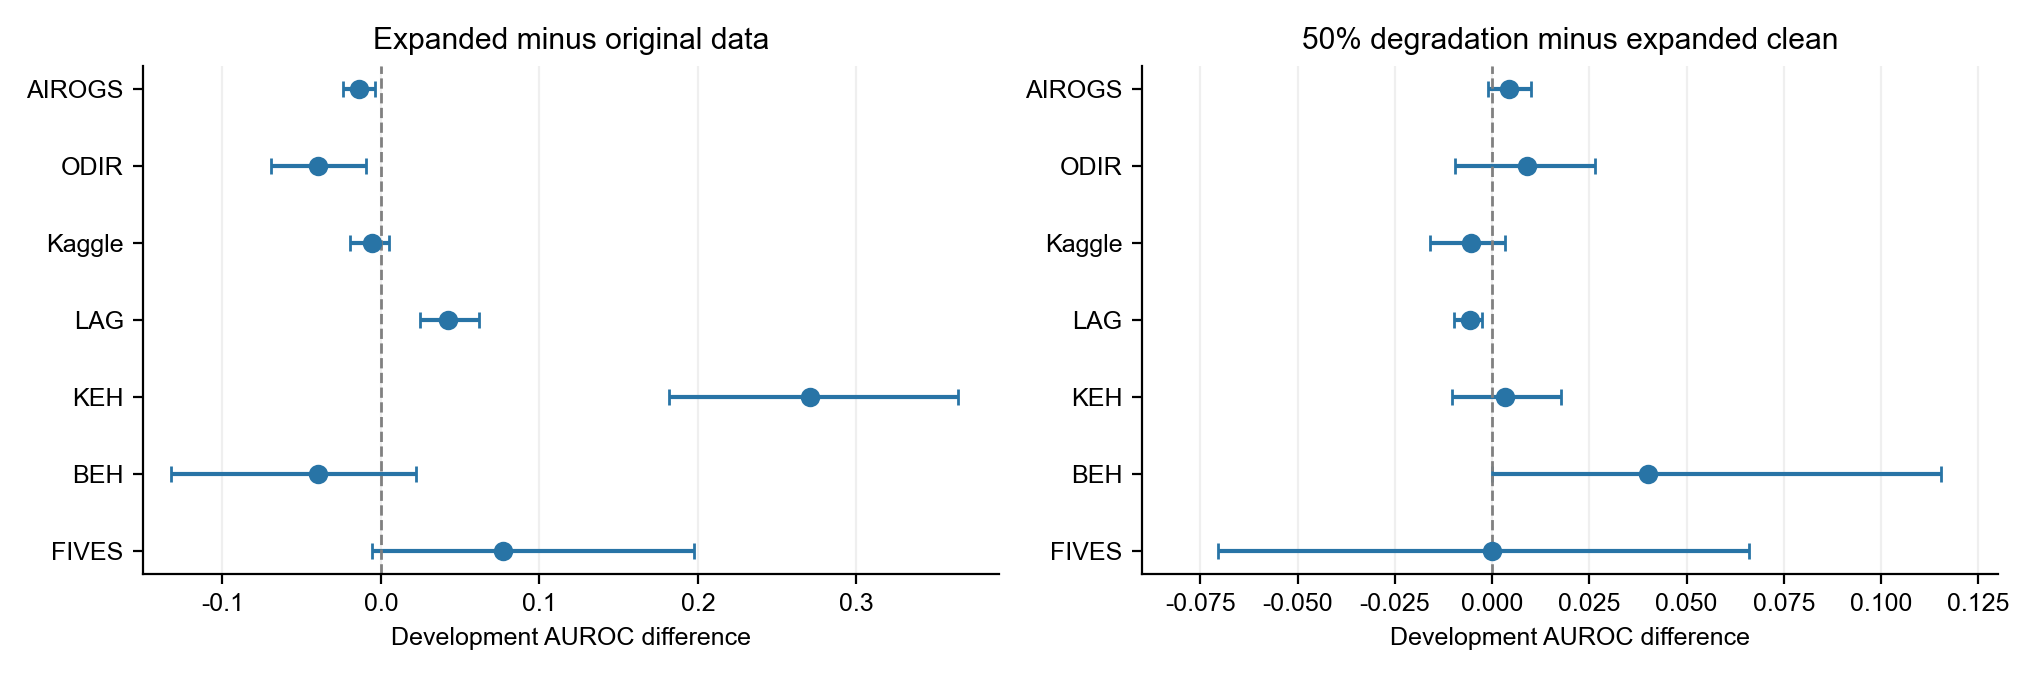
\includegraphics[keepaspectratio,alt={Paired source AUROC differences at update 1,200}]{source-differences.en.png}}
\caption{Paired source AUROC differences at update 1,200}
\end{figure}

Figure 1 compares expanded clean with original data on the left and 50\%
degradation with expanded clean on the right. Points show AUROC
differences, horizontal bars linked-group 95\% intervals, and dashed
lines zero difference. The panels use different horizontal ranges to
show their respective changes clearly. Adding 50\% degradation reduces
LAG original-image AUROC by 0.0058 {[}−0.0098, −0.0025{]}; the AIROGS,
ODIR, and KEH additional-change intervals include zero.

AUPRC is the area under the precision--recall curve. It describes
precision and coverage of positive detections, varies with source
prevalence, and supports comparisons within a source. The Brier score is
the mean squared difference between predicted probabilities and 0/1
labels; lower values indicate more accurate probability predictions.

\Needspace{12\baselineskip}
\begin{longtable}[]{@{}
  >{\raggedright\arraybackslash}p{(\linewidth - 4\tabcolsep) * \real{0.2727}}
  >{\raggedleft\arraybackslash}p{(\linewidth - 4\tabcolsep) * \real{0.3636}}
  >{\raggedleft\arraybackslash}p{(\linewidth - 4\tabcolsep) * \real{0.3636}}@{}}
\toprule\noalign{}
\begin{minipage}[b]{\linewidth}\raggedright
Update 1,200: expansion − original
\end{minipage} & \begin{minipage}[b]{\linewidth}\raggedleft
AUPRC difference {[}95\% interval{]}
\end{minipage} & \begin{minipage}[b]{\linewidth}\raggedleft
Brier difference {[}95\% interval{]}
\end{minipage} \\
\midrule\noalign{}
\endhead
\bottomrule\noalign{}
\endlastfoot
AIROGS & -0.0123 {[}-0.0231, -0.0023{]} & +0.0230 {[}+0.0110,
+0.0356{]} \\
ODIR & -0.1604 {[}-0.2920, +0.0104{]} & +0.0217 {[}+0.0027,
+0.0412{]} \\
LAG & +0.0735 {[}+0.0404, +0.1118{]} & -0.0571 {[}-0.0811, -0.0330{]} \\
KEH & +0.2578 {[}+0.1561, +0.3600{]} & -0.1482 {[}-0.1998, -0.0973{]} \\
\end{longtable}

KEH and LAG improve in AUPRC and Brier, while AIROGS worsens in both,
consistent with their AUROC directions. ODIR Brier increases, but its
AUPRC difference interval includes zero. The 305 ODIR development images
represent only 193 linked groups, including 19 positive groups,
contributing to wider positive-detection intervals.

\subsection{How added sources affect sampling and checkpoint
selection}\label{how-added-sources-affect-sampling-and-checkpoint-selection}

Each optimizer update processes a sampled batch; an image can appear
several times during training. The current sampler assigns each image
the inverse square root of the number of images in its source-and-class
combination. Larger combinations receive more total sampling weight, but
the weight grows more slowly than image count. Adding sources reduces
the sampling share allocated to original sources.

\Needspace{12\baselineskip}
\begin{longtable}[]{@{}
  >{\raggedright\arraybackslash}p{(\linewidth - 4\tabcolsep) * \real{0.2727}}
  >{\raggedleft\arraybackslash}p{(\linewidth - 4\tabcolsep) * \real{0.3636}}
  >{\raggedleft\arraybackslash}p{(\linewidth - 4\tabcolsep) * \real{0.3636}}@{}}
\toprule\noalign{}
\begin{minipage}[b]{\linewidth}\raggedright
Arm
\end{minipage} & \begin{minipage}[b]{\linewidth}\raggedleft
Original presentations / distinct images
\end{minipage} & \begin{minipage}[b]{\linewidth}\raggedleft
Added presentations / distinct images
\end{minipage} \\
\midrule\noalign{}
\endhead
\bottomrule\noalign{}
\endlastfoot
Original & 19,186/8,339 & 0/0 \\
Expanded & 9,484/5,929 & 9,708/3,901 \\
30\% degradation & 9,484/5,929 & 9,708/3,901 \\
50\% degradation & 9,484/5,929 & 9,708/3,901 \\
\end{longtable}

Distinct images in the table are images presented at least once.
Original training makes 19,186 presentations, covering 8,339/10,338
training images (80.7\%). Expanded training makes 9,484 original-image
presentations, or 49.4\%, covering 5,929 original images (57.4\%). Added
images contribute 9,708 presentations, or 50.6\%, covering 3,901/5,142
added training images (75.9\%). All three expanded arms have identical
per-image presentation counts, supporting the augmentation comparison.
Partial final batches cause the six-presentation difference in totals.

A single added image appears up to 30 times, versus 14 for original
training. Expansion changes source composition, original-image
presentations, and repetition frequency together. Controlling the
original-image quota in the next round will help assess their effects on
original-source performance.

\begin{figure}[H]
\centering
\pandocbounded{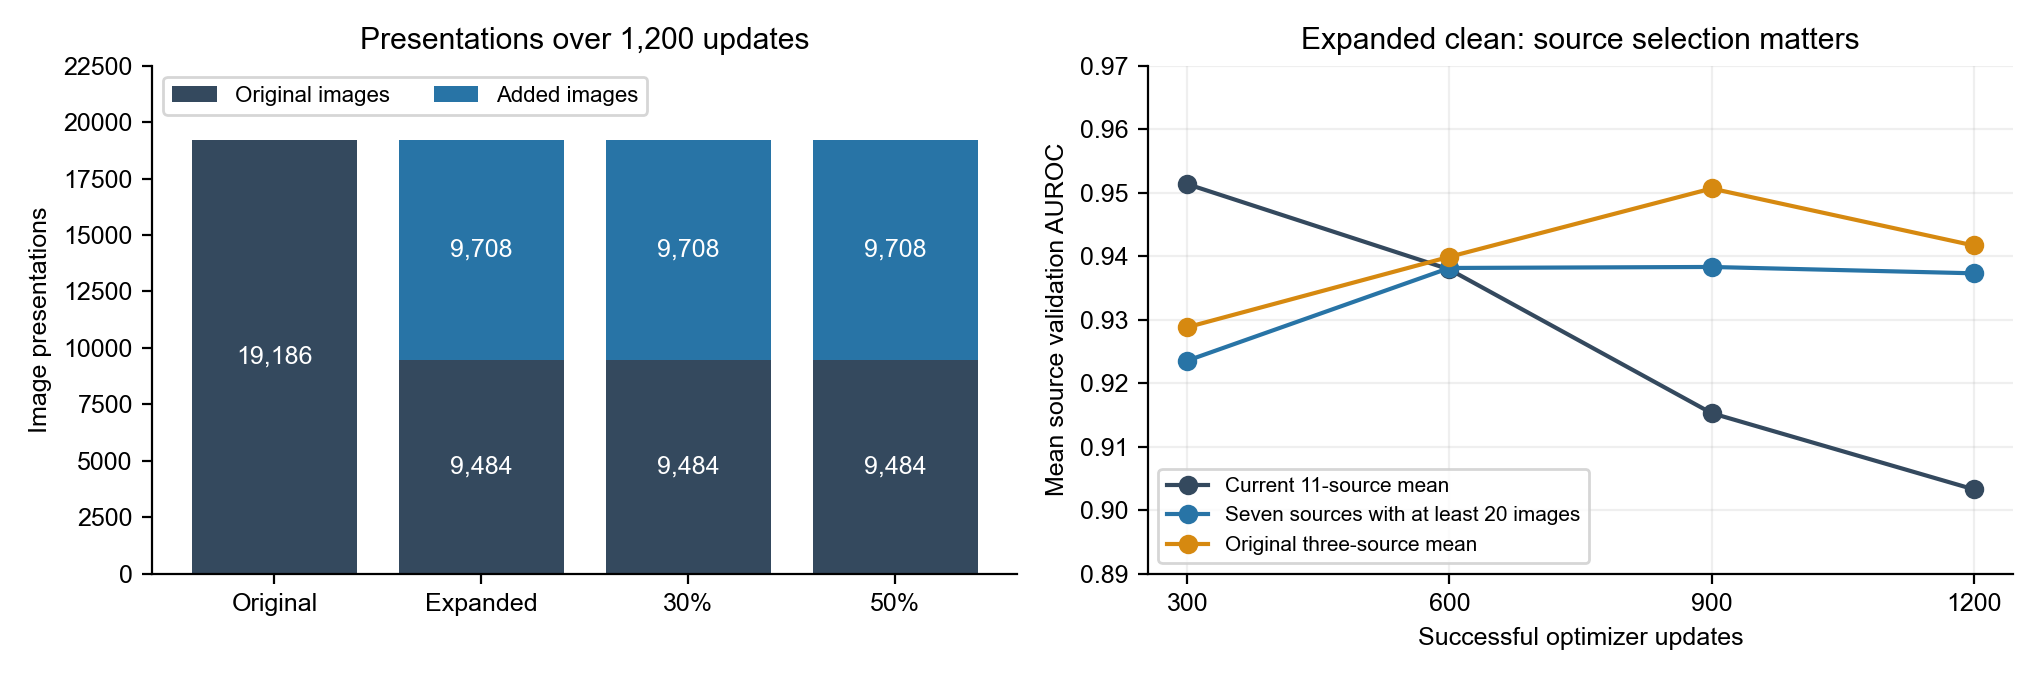
\includegraphics[keepaspectratio,alt={Actual image presentations and changes in validation means}]{exposure-selection.en.png}}
\caption{Actual image presentations and changes in validation means}
\end{figure}

Figure 2 shows original and added image presentations on the left and
expanded-clean validation AUROC means over three source combinations on
the right. This round selects checkpoints using an equal mean over 11
validation sources containing both classes. HRF, CRFO, Fundus-AVSeg, and
LES-AV have just 4, 6, 3, and 2 validation images: 15 images account for
4/11, or 36.4\%, of that mean's weight.

Between updates 300 and 1,200, expanded-clean HRF AUROC falls from 1.0
to 0.5, reducing the 11-source mean by 0.04545; the total decline is
0.04807. CRFO contributes another −0.01136, partly offset by
other-source gains. In original training, CRFO rises from 0.5 to 1.0 and
contributes +0.04545, compared with a total mean gain of 0.03241. A few
validation images consequently have substantial influence on checkpoint
selection.

Considering only the seven sources with at least 20 validation images,
the expanded-clean mean rises from 0.9235 to 0.9373 and peaks at update
900. The original three-source mean also peaks at 900. This sensitivity
analysis uses existing validation logs. Full update-600 and update-900
checkpoints were not saved, so development results use the saved
update-300 and update-1,200 weights.

\subsection{Effects of augmentation under synthetic
defocus}\label{effects-of-augmentation-under-synthetic-defocus}

Synthetic degradation evaluation uses the same 384 development
originals: 146 positives and 238 negatives, selected deterministically
by image-identifier hashes. Defocus uses radius 2 for a 512-pixel fundus
field, scaled to the actual field. Exposure variants multiply brightness
by 0.70. Originals and degraded versions are paired. The table uses
update-1,200 weights and labels an image positive when its probability
exceeds 0.5, the display threshold for this round.

\Needspace{12\baselineskip}
\begin{longtable}[]{@{}
  >{\raggedright\arraybackslash}p{(\linewidth - 8\tabcolsep) * \real{0.3571}}
  >{\raggedleft\arraybackslash}p{(\linewidth - 8\tabcolsep) * \real{0.1607}}
  >{\raggedleft\arraybackslash}p{(\linewidth - 8\tabcolsep) * \real{0.1607}}
  >{\raggedleft\arraybackslash}p{(\linewidth - 8\tabcolsep) * \real{0.1607}}
  >{\raggedleft\arraybackslash}p{(\linewidth - 8\tabcolsep) * \real{0.1607}}@{}}
\toprule\noalign{}
\begin{minipage}[b]{\linewidth}\raggedright
Condition / measure
\end{minipage} & \begin{minipage}[b]{\linewidth}\raggedleft
Original
\end{minipage} & \begin{minipage}[b]{\linewidth}\raggedleft
Expanded
\end{minipage} & \begin{minipage}[b]{\linewidth}\raggedleft
30\%
\end{minipage} & \begin{minipage}[b]{\linewidth}\raggedleft
50\%
\end{minipage} \\
\midrule\noalign{}
\endhead
\bottomrule\noalign{}
\endlastfoot
Original: AUROC & 0.9423 & 0.9690 & 0.9702 & 0.9688 \\
Original: misses / false positives & 30/16 & 23/15 & 21/13 & 23/14 \\
Defocus: AUROC & 0.9193 & 0.8894 & 0.9332 & 0.9449 \\
Defocus: misses / false positives & 55/10 & 18/68 & 36/23 & 28/19 \\
Exposure 0.70: AUROC & 0.9382 & 0.9536 & 0.9611 & 0.9564 \\
Exposure 0.70: misses / false positives & 39/13 & 21/23 & 26/17 &
29/18 \\
\end{longtable}

Under defocus, 50\% degradation improves AUROC by 0.0555 {[}0.0308,
0.0817{]} and AUPRC by 0.1019 {[}0.0511, 0.1592{]}, and reduces Brier by
0.0684 {[}0.0445, 0.0938{]}, relative to expanded clean. False positives
fall from 68/238 to 19/238: a 20.59-percentage-point reduction {[}15.25,
26.03{]}. Misses rise from 18/146 to 28/146: a 6.85-point increase
{[}0.71, 13.33{]}. Ranking gains and the missed-positive/false-positive
balance at a fixed threshold should be assessed together.

\begin{figure}[H]
\centering
\pandocbounded{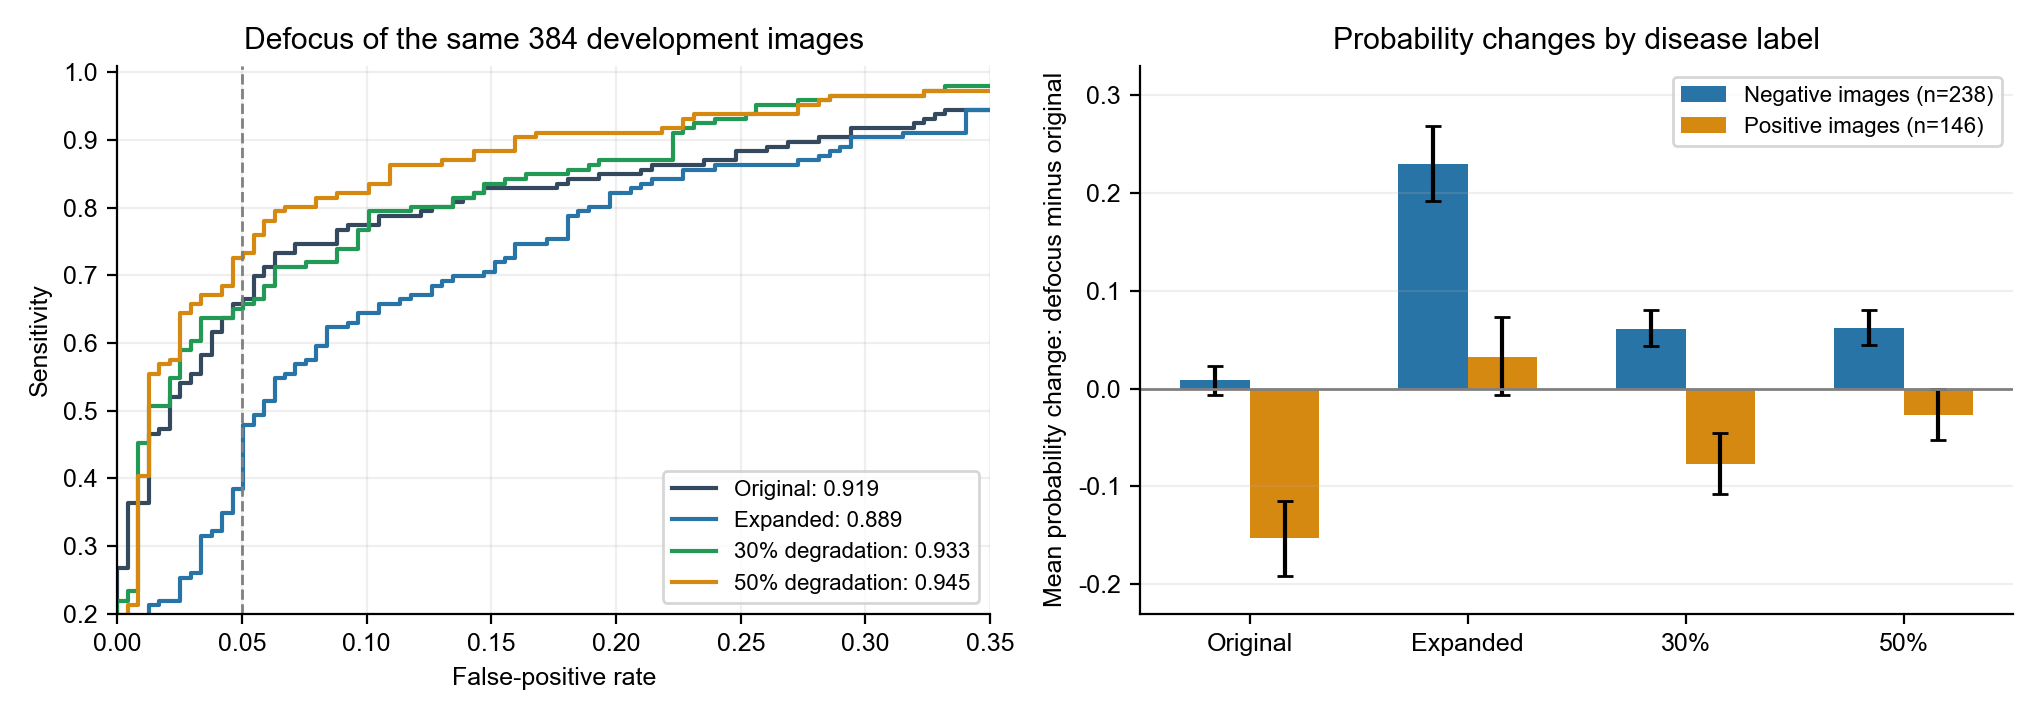
\includegraphics[keepaspectratio,alt={ROC curves and probability changes under synthetic defocus}]{defocus-ranking-shifts.en.png}}
\caption{ROC curves and probability changes under synthetic defocus}
\end{figure}

Figure 3 shows sensitivity versus false-positive rate over thresholds on
the left, with AUROC in the legend. The right panel shows mean
defocus-minus-original probability changes by disease label with 95\%
intervals. Expanded-clean negative scores rise by 0.2295 on average,
versus 0.0622 with 50\% degradation. Original-training positive scores
fall by 0.1523, versus 0.0273 with 50\% degradation. Augmentation
reduces the effect of defocus on both classes' scores.

Matching specificity at 95.4\% on the same degraded subset gives defocus
sensitivities of 65.8\%, 38.4\%, 65.1\%, and 72.6\%. This exploratory
comparison recalculates thresholds for each arm and condition to explain
ranking. Within-source comparisons also show gains: adding 50\%
degradation improves defocused AIROGS AUROC by 0.0691 {[}0.0258,
0.1149{]} and LAG by 0.0835 {[}0.0341, 0.1455{]}.

A separate comparison fixes each arm's source thresholds from original
validation negatives and applies them to original and degraded images.
Seven sources with both validation classes contribute 356
stress-evaluation images: 139 positives and 217 negatives. The other 28
images come from small sources missing one validation class. Entries
below are misses / false positives.

\Needspace{12\baselineskip}
\begin{longtable}[]{@{}
  >{\raggedright\arraybackslash}p{(\linewidth - 8\tabcolsep) * \real{0.3571}}
  >{\raggedleft\arraybackslash}p{(\linewidth - 8\tabcolsep) * \real{0.1607}}
  >{\raggedleft\arraybackslash}p{(\linewidth - 8\tabcolsep) * \real{0.1607}}
  >{\raggedleft\arraybackslash}p{(\linewidth - 8\tabcolsep) * \real{0.1607}}
  >{\raggedleft\arraybackslash}p{(\linewidth - 8\tabcolsep) * \real{0.1607}}@{}}
\toprule\noalign{}
\begin{minipage}[b]{\linewidth}\raggedright
Condition: fixed validation thresholds
\end{minipage} & \begin{minipage}[b]{\linewidth}\raggedleft
Original
\end{minipage} & \begin{minipage}[b]{\linewidth}\raggedleft
Expanded
\end{minipage} & \begin{minipage}[b]{\linewidth}\raggedleft
30\%
\end{minipage} & \begin{minipage}[b]{\linewidth}\raggedleft
50\%
\end{minipage} \\
\midrule\noalign{}
\endhead
\bottomrule\noalign{}
\endlastfoot
Original & 34/11 & 27/7 & 30/10 & 30/11 \\
Defocus & 63/10 & 28/47 & 45/16 & 40/10 \\
Exposure 0.70 & 38/8 & 25/15 & 30/13 & 35/13 \\
\end{longtable}

At fixed validation thresholds, adding 50\% degradation reduces defocus
false positives from 47 to 10 and increases misses from 28 to 40. With
exposure multiplied by 0.70, the AUROC difference is +0.0028 {[}−0.0078,
0.0138{]} and misses increase from 25 to 35. Current augmentation gains
concentrate on defocus. Separating defocus-only from mixed augmentation
in the next round will help identify useful degradation types and
strengths.

\subsection{Real poor-quality detections and label
distribution}\label{real-poor-quality-detections-and-label-distribution}

Real poor-quality development images comprise seven FIVES and five MSHF
positives in 12 distinct linked groups. At threshold 0.5, original
training detects 7/12, and all three expanded arms detect 12/12. The
exact binomial 95\% interval for 12/12 is 73.5\%--100\%; FIVES and MSHF
intervals are 59.0\%--100\% and 47.8\%--100\%, respectively. Five
additional detections comprise two FIVES and three MSHF images, with no
additional misses. The exact McNemar test of changed decisions on the
same images gives two-sided p=0.0625. The intervals indicate substantial
sampling uncertainty for this small set.

\begin{figure}[H]
\centering
\pandocbounded{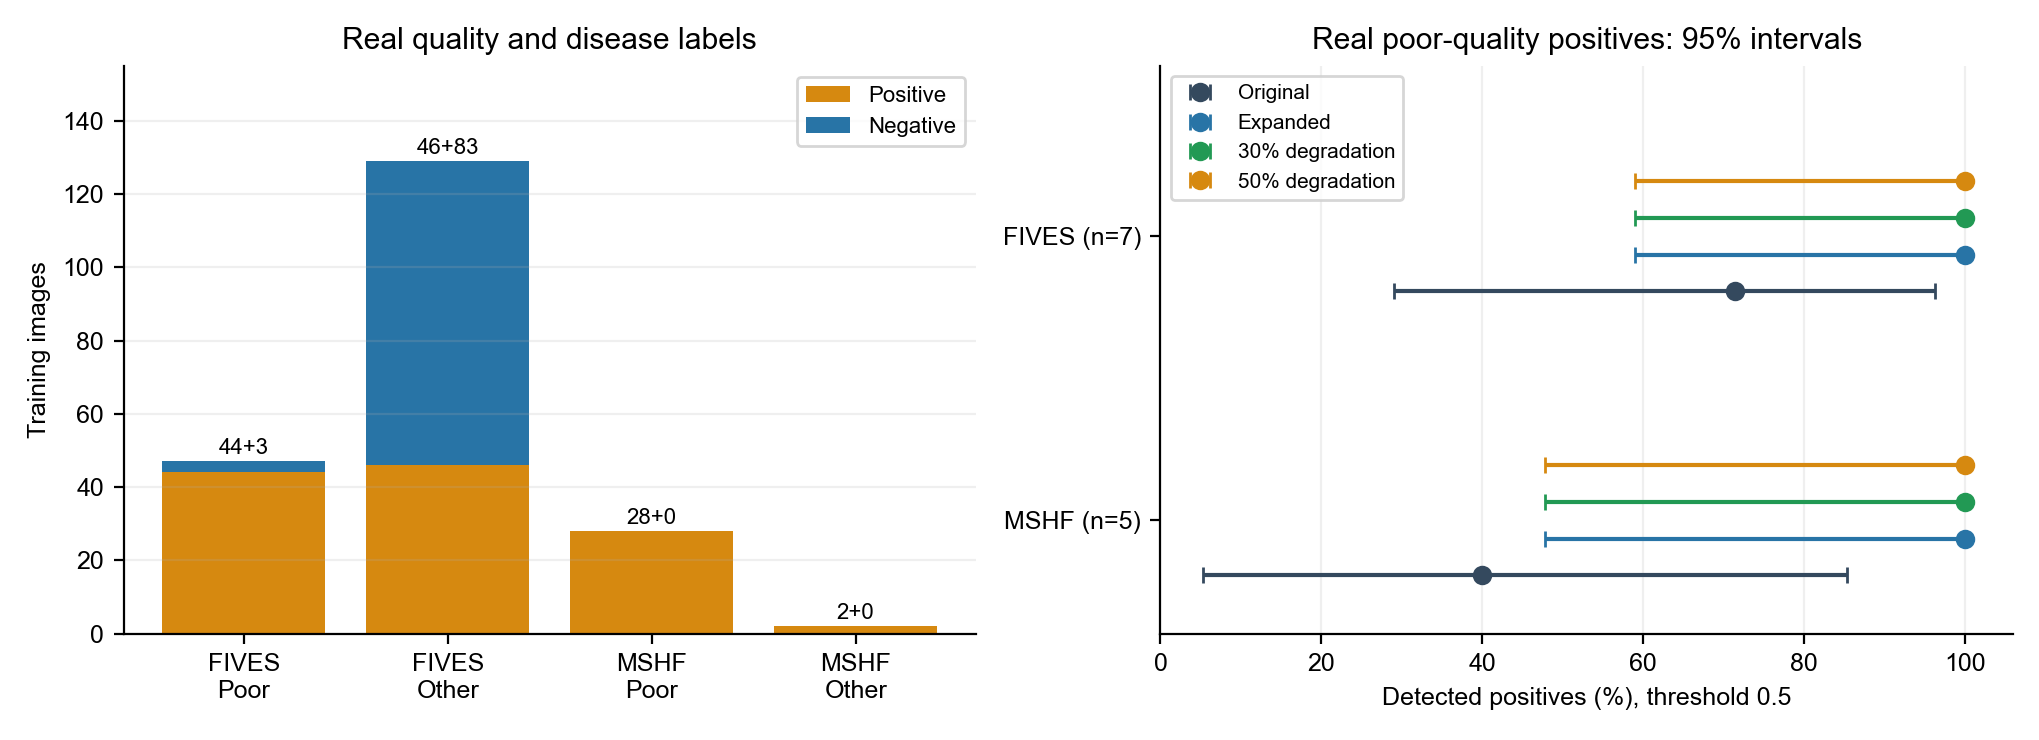
\includegraphics[keepaspectratio,alt={Training distribution of real quality and disease labels, and development detections}]{real-quality-labels.en.png}}
\caption{Training distribution of real quality and disease labels, and
development detections}
\end{figure}

Figure 4 shows training-image counts by source and original quality
annotation on the left; labels above bars are positive + negative
counts. The right panel shows detected proportions and exact binomial
95\% intervals for each source's real poor-quality development
positives. FIVES defines poor quality as at least one poor quality
dimension, while MSHF uses overall quality. Other quality covers each
source's remaining grades; source-specific annotation standards are
retained.

Of 47 poor-quality FIVES training images, 44 are positive and three
negative. Its other 129 images contain 46 positives and 83 negatives.
All 28 poor-quality and two other-quality MSHF training images are
positive. Actual training includes 413 poor-quality positive
presentations from these sources and only ten negative presentations.
Given this association between quality and disease labels, the next
round should add same-source poor-quality negatives and compare
quality-balanced sampling to distinguish source and quality cues from
disease features.

At fixed source thresholds from validation, expanded clean and 50\%
degradation both detect all seven poor-quality FIVES positives.
Comparing these arms, sensitivity over all 13 FIVES development
positives rises from 76.9\% to 92.3\%, while specificity on 14 negatives
falls from 100\% to 78.6\%. Thresholds come from just 14 validation
negatives and select their maximum score; additional negatives are
needed to stabilize threshold estimates. MSHF currently contains
positives only, so source-specific specificity requires added negatives.

\subsection{Proposed next controlled
experiment}\label{proposed-next-controlled-experiment}

Use one original-data control and four expanded arms combining two
sampling methods, current sampling and a 65\% original-image quota, with
two augmentation settings, no degradation and 50\% mixed degradation.
Use three common seeds, equal initialization conditions, and 2,400
successful updates per arm. At 16 images per batch, the 65\% quota
provides about 24,960 original-image presentations, versus 19,186 in
this round's control. Retain inverse-square-root weights within sources.
Compare sampling and augmentation at equal budgets, and save
update-1,200 and update-2,400 checkpoints to assess continued training.

Predeclare the equal AUROC mean over AIROGS, ODIR, Kaggle, LAG, and KEH
as the primary checkpoint-selection criterion. Report the original
three-source mean and source-specific sensitivity and specificity as
well. Treat BEH, FIVES, and smaller sources as supplementary
evaluations. Save full weights and predictions every 300 updates, and
report development-image bootstrap intervals separately from variation
across seeds.

Then compare defocus-only with mixed augmentation using the same
application probability, sampling sequence, and update budget. Evaluate
misses, false positives, real poor-quality negatives, and original-image
AUROC and Brier at fixed validation thresholds. Use predeclared
original-source performance, quality-stratified results, and review
workload to select models and thresholds before final testing. These are
proposed experiments and have not yet run.

\subsection{Analysis artifacts and
reproduction}\label{analysis-artifacts-and-reproduction}

\href{../training-results/training-results.en.md}{Training results} ·
\href{../training-results/data-audit.en.md}{Data audit} ·
\href{../training-results/degradation-audit.en.md}{Degradation audit} ·
\href{training-exposure.json}{Image presentation counts} ·
\href{figure-data.json}{Figure data} ·
\href{../../../../tools/analyze_expansion_results_20261113.py}{Analysis
program} ·
\href{../../../../tools/report_expansion_analysis_20261113.py}{Report
generator}

Run the analysis program with \texttt{-\/-extract-draws} in the training
environment to extract per-image presentation counts from checkpoints.
Then run the analysis and report programs in the document environment.
The analysis checks image identifiers, labels, sources, linked groups,
and frozen-manifest metadata for all four arms, retaining input SHA256
hashes. Statistical tests cover tied scores, linked-group resampling,
and same-image pairing.

\end{document}
